%
% normbeispiele.tex
%
% (c) 2023 Prof Dr Andreas Müller
%
\begin{figure}
\centering
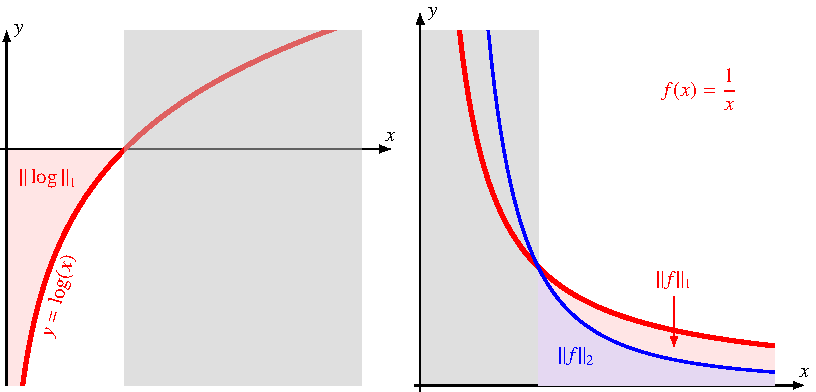
\includegraphics{chapters/010-skalarprodukt/images/normbeispiele.pdf}
\caption{Beispiele von Funktionen, für die nicht alle Normen überhaupt
einen wohldefinierten Wert haben.
Links die Logarithmusfunktion, die auf dem Intervall $[0,1]$ zwar
eine beschränkte $L^1$-Norm hat, aber unbeschränkte Supremum-Norm.
Rechts ist Funktion $f(x)=1/x$ dargestellt, die auf dem Intervall
$[0,\infty)$ eine beschränkte $L^2$-Norm hat, während die $L^1$-Norm
unbeschränkt ist.
\label{buch:skalarprodukt:funktionenraeume:fig:normbeispiele}}
\end{figure}
